\documentclass{article}
\usepackage[margin=1in]{geometry}
\usepackage{amsmath,amsthm,amssymb}
\usepackage{bbm,enumerate,mathtools}
\usepackage{tikz,pgfplots}
\usepackage{chessboard}
\usepackage[hidelinks]{hyperref}
\usepackage{multicol} % Problem 35
\usepackage{xstring} % Difficulty command
\usetikzlibrary{shapes.geometric}

\newenvironment{question}{\begin{trivlist}\item[\textbf{Question.}]}{\end{trivlist}}
\newenvironment{note}{\begin{trivlist}\item[\textbf{Note.}]}{\end{trivlist}}
\newenvironment{references}{\begin{trivlist}\item[\textbf{References.}]}{\end{trivlist}}
\newenvironment{related}{\begin{trivlist}\item[\textbf{Related.}]\end{trivlist}\begin{enumerate}}{\end{enumerate}}

\newcommand\score[1]{
\pgfmathsetmacro\pgfxa{#1+1}
\tikzstyle{scorestars}=[
  star,
  star points=5,
  star point ratio=2.25,
  draw,
  inner sep=3pt,
  anchor=outer point 5
]
  \begin{tikzpicture}[baseline]
    \draw[opacity=0] (0,-0.5) rectangle (0,0.2); % Workaround for whitespace at the bottom.
    \foreach \i in {1,...,4} {
      \pgfmathparse{(\i<=#1?"yellow":"gray")}
      \edef\starcolor{\pgfmathresult}
      \draw (\i*4.5ex,0) node[name=star\i,scorestars,fill=\starcolor]  {};
    }
  \end{tikzpicture}
}

\newcommand{\difficulty}[1]{%
  \IfEqCase{#1}{%
      {1}{
        
\begin{tikzpicture}[scale=0.7, baseline=0.9mm]%
          \definecolor{slopegreen}{rgb}{0.0, 0.5, 0.0}%
          \fill[slopegreen] (0.5,0.5) circle (0.5);%
        \end{tikzpicture}%
      }%
      {2}{
        
\begin{tikzpicture}[scale=0.7, baseline=0.9mm]%
          \definecolor{slopeblue}{rgb}{0.0, 0.44, 1.00}
          \fill[slopeblue] (0,0) rectangle (1,1);%
        \end{tikzpicture}%
      }%
      {3}{
\begin{tikzpicture}[scale=0.7, baseline=0.9mm]\fill (0,0.5)--(0.5, 0)--(1,0.5)--(0.5,1)--cycle; \end{tikzpicture}}%
      {4}{
\begin{tikzpicture}[scale=0.7, baseline=0.9mm]\fill (0.25,0)--(0,0.5)--(0.25,1)--(0.5,0.5)--cycle; \fill (0.75,0)--(0.5,0.5)--(0.75,1)--(1,0.5)--cycle;\end{tikzpicture}}%
      % you can add more cases here as desired
  }[\PackageError{difficulty}{Undefined difficulty level: #1}{}]%
}%
\newcommand{\rating}[2]{\difficulty{#1}\\\score{#2}\\}


\begin{document}

\rating{2}{2}
Consider attempting to fill in a $n \times n$ Latin square with the numbers $1$
through $n$, one number at a time. A clumsy filling is an incomplete filling in
which no more valid moves are possible.
\begin{figure}[ht!]
  \centering
  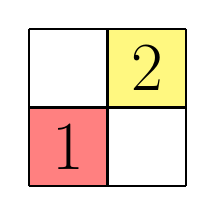
\begin{tikzpicture}
    \foreach \x/\y/\n/\c in {
      1/1/1/red,
      2/2/2/yellow}
    {
      \fill[\c!50] (\x - 1, \y - 1) rectangle (\x, \y);
      \node at (\x - 0.5, \y - 0.5) {\Huge\n};
    }
    \draw[thick] (0,0) grid (2,2);
  \end{tikzpicture}
  \\~\\
  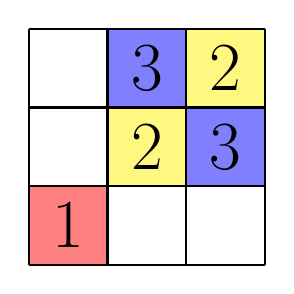
\begin{tikzpicture}
    \foreach \x/\y/\n/\c in {
      1/1/1/red,
      2/2/2/yellow, 2/3/3/blue,
      3/2/3/blue, 3/3/2/yellow}
    {
      \fill[\c!50] (\x - 1, \y - 1) rectangle (\x, \y);
      \node at (\x - 0.5, \y - 0.5) {\Huge\n};
    }
    \draw[thick] (0,0) grid (3,3);
  \end{tikzpicture}
  ~~~
  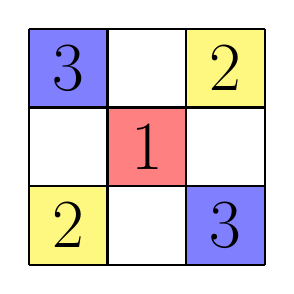
\begin{tikzpicture}
    \foreach \x/\y/\n/\c in {
      1/1/2/yellow, 1/3/3/blue,
      2/2/1/red,
      3/1/3/blue, 3/3/2/yellow}
    {
      \fill[\c!50] (\x - 1, \y - 1) rectangle (\x, \y);
      \node at (\x - 0.5, \y - 0.5) {\Huge\n};
    }
    \draw[thick] (0,0) grid (3,3);
  \end{tikzpicture}
  \\~\\
  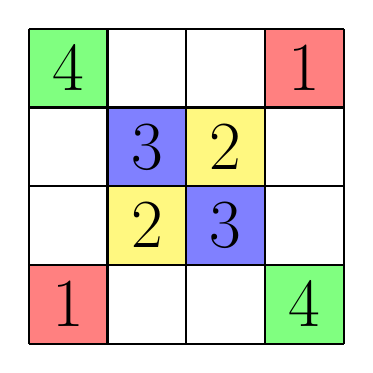
\begin{tikzpicture}
    \foreach \x/\y/\n/\c in {
      1/1/1/red, 1/4/4/green,
      2/2/2/yellow, 2/3/3/blue,
      3/2/3/blue, 3/3/2/yellow,
      4/1/4/green, 4/4/1/red}
    {
      \fill[\c!50] (\x - 1, \y - 1) rectangle (\x, \y);
      \node at (\x - 0.5, \y - 0.5) {\Huge\n};
    }
    \draw[thick] (0,0) grid (4,4);
  \end{tikzpicture}
  ~~~
  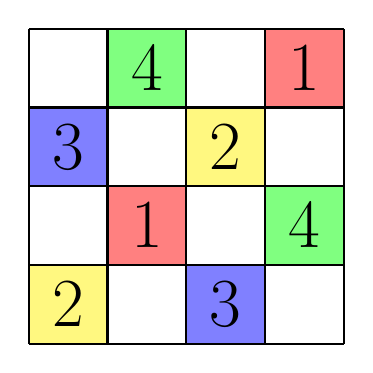
\begin{tikzpicture}
    \foreach \x/\y/\n/\c in {
      1/1/2/yellow, 1/3/3/blue,
      2/2/1/red, 2/4/4/green,
      3/1/3/blue, 3/3/2/yellow,
      4/2/4/green, 4/4/1/red}
    {
      \fill[\c!50] (\x - 1, \y - 1) rectangle (\x, \y);
      \node at (\x - 0.5, \y - 0.5) {\Huge\n};
    }
    \draw[thick] (0,0) grid (4,4);
  \end{tikzpicture}
  \caption{
    Clumsy filling for $n=2,3,4$ can be achieved with $2$, $5$, and $8$ or fewer entries respectively;
    thus $a(2) = 2, a(4) \leq 5,$ and $a(4) \leq 8$.
  }
\end{figure}

\begin{question}
  Let $a(n)$ be the fewest number of entries required for a clumsy filling.
  What is $a(n)$?
\end{question}

\begin{related}
  \item How many ``essentially different'' fillings are there? \\
  (Two fillings are the same if related by permuting the symbols or
  dihedral action of the board.)
  \item Can minimal clumsy fillings be built iteratively, as suggested by the
  leftmost diagrams in the example?
  \item What if this is done on a group table instead of a Latin square
  (quasigroup table)?
\end{related}

\end{document}
